\documentclass[10pt, a4paper]{article}
\usepackage[utf8]{inputenc}
\usepackage[T1]{fontenc,url}
\usepackage{multicol}
\usepackage{multirow}
\usepackage{parskip}
\usepackage{lmodern}
\usepackage{microtype}
\usepackage{verbatim}
\usepackage{amsmath, amssymb}
\usepackage{tikz}
\usepackage{physics}
\usepackage{mathtools}
\usepackage{algorithm}
\usepackage{algpseudocode}
\usepackage{listings}
\usepackage{enumerate}
\usepackage{graphicx}
\usepackage{float}
\usepackage{hyperref}
\usepackage{tabularx}
\usepackage{siunitx}
\usepackage{fancyvrb}
%\usepackage{natbib}
%\bibliographystyle{dinat}
\usepackage[makeroom]{cancel}
\usepackage[margin=2.0cm]{geometry}
\usepackage{pdfpages}
\usepackage[margin=10pt, textfont={small, it}, labelfont={bf}, labelsep=endash]{caption}
\renewcommand{\baselinestretch}{1}

\begin{document}
\title{COMAP - Compression of level 1 files}
\author{
    \begin{tabular}{r l}
        Jonas Gahr Sturtzel Lunde & (\texttt{jonassl@astro.uio.no})
    \end{tabular}}
% \date{}    % if commented out, the date is set to the current date
\maketitle
Relevant code found at \url{https://github.com/asdfbat/comap_compress}
\vspace{0.7cm}

\section*{Summary}
Compression of a 50-60GB 1 hour obervation, using the suggested GZIP level 3 compression:
\begin{itemize}
    \item Compression time: $\sim$ 80 minutes
    \item Compression ratio: $\sim$ 1.9
    \item Decompression time: $\sim$ 6 minutes
\end{itemize}

The hdf5 library contains support for compressed files, which we can use to reduce the storage requirements of our level 1 files. A typical level 1 file, consisting of a 1 hour obervation, is of the size 50-60GB, which can be reduced by a factor of around 1.9 through lossless compression. The compression takes somewhat over an hour to perform on a typical processor core. The compression itself is not parallelizable, but multiple compressions can be run in parallel. Once compressed, the .h5 files function as normal, and will be automatically decompressed once read. The decompression typically takes 6 minutes per file.


\section*{Implementation}
The compression can be done with the h5repack command:

\texttt{h5repack -f /spectrometer/tod:GZIP=3 oldfile.hd5 newfile.hd5}

We can specify that only parts of the hdf5 hierarchy be compressed, as done above with \texttt{/spectrometer/tod}. We do this because over $99\%$ of the data is in this single data field, making compression of other quantities meaningless. We can also specify a level of GZIP compression in the range 1-9, where we have in the above example selected 3.

\section*{Compression level}
h5repack offers compression levels in the range of 1-9. The figures below show its impact on compression ratio, compression time, and decompression time. GZIP levels above 5 are not shown, as the compression times of these levels were ridiculous, without meaningful gain in other areas.

My suggestion, based on these results, is to employ the level 3 GZIP compression, which seems to be very well suited for our needs. It offers both the highest compression ratio and lowest decompression time among the considered levels, without the unreasonable compression times offered by levels 5 and above. Level 1 is also a reasonable choice, but as the compression is only performed once, it seems worth it to sacrifice some compression time for better compression ratio and decompression time.

\begin{figure}[H]
    \centering
    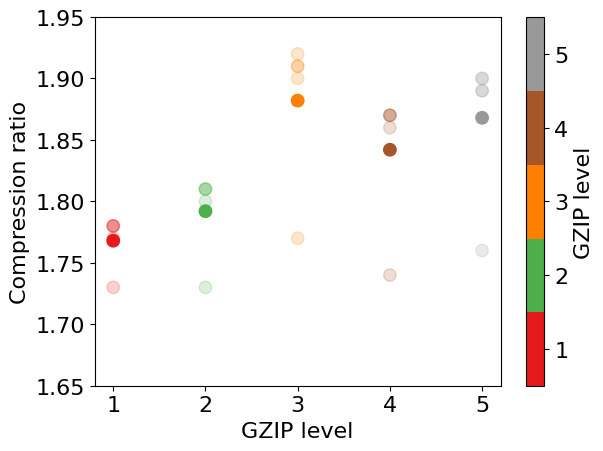
\includegraphics[scale=0.55]{gzip_compratio.png}
    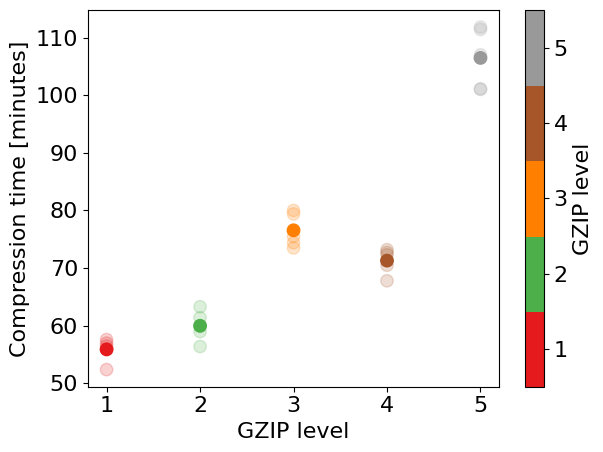
\includegraphics[scale=0.55]{gzip_comptime.png}
    \caption{Compression ratio (left) and compression time (right) of 5 random 50-60GB observations, as function of GZIP level. The mean of the 5 points are shown as a solid dot.}
    \label{fig:fig1}
\end{figure}

\begin{figure}[H]
    \centering
    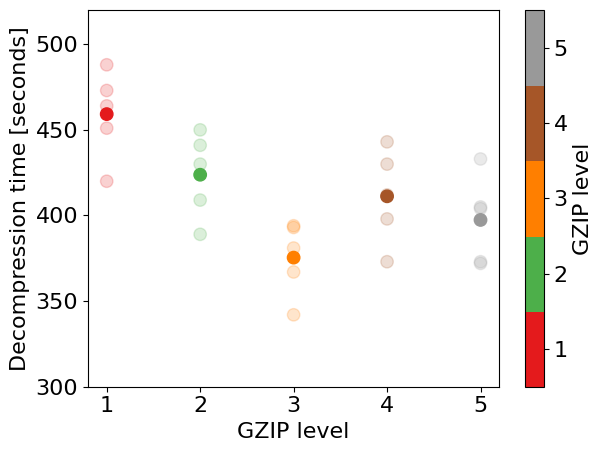
\includegraphics[scale=0.55]{gzip_decomptime.png}
    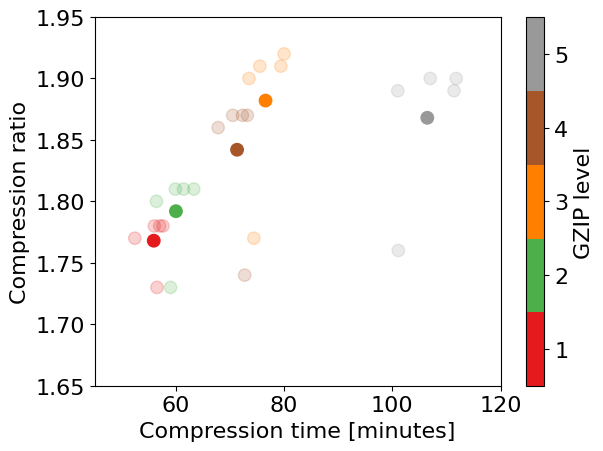
\includegraphics[scale=0.55]{comptime_compratio.png}
    \caption{Decompression time as function of GZIP level (left), and relation between compression time and compression ratio (right) of 5 random 50-60GB observations. The mean of the 5 points are shown as a solid dot.}
    \label{}
\end{figure}


\section*{Other parameters}
A number of other parameters can be tuned when compressing files with h5repack. One can, among other things, change the compression algorithm to something other than GZIP, or adjust the chunk size of the chunking layout of the data. I found all things I tried to give either identical or much worse results. One thing to consider is that the entire compressed TOD is always read in its entirety, removing the need for a compression which performs well on random reads.

In summary, my limited testing found no need to set any other parameters than the GZIP level.

\end{document}